\documentclass[letterpaper,12pt]{article}
\usepackage[utf8]{inputenc}
\usepackage[russian]{babel}
\usepackage[left=2cm,right=2cm,top=2cm,bottom=2cm,bindingoffset=0cm]{geometry}
\usepackage{graphicx}
\graphicspath{{images/}}
\usepackage{float}
\usepackage{wrapfig}


\begin{document}
\begin{center}
Описание возможных случаев поведения алгоритма в процессе <<перешагивания>>
ребра
\end{center}
Как входные данные имеем: 
\begin{enumerate}
      \item Контейнер упорядоченных по полярному углу относительно
            прошлой грани точек.
      \item Индексы $i, j$ точек, задающих <<перешагиваемое>> ребро.
      \item Отрезки, концами которых являются данные точки.
      \item Информация о правильности затронутых отрезков.
\end{enumerate}
Не умоляя общности, рассмотрим случаи для ребра расположенного вертикально:
\begin{enumerate}
      \item Точки $p_i, p_j$ являются точками одного отрезка. Так как
            варианты с <<перешагиванием>> отрезка исключены из рассмотрения,
            вожможен только изображенный ниже случай и его зеркальная версия.
            
            Действие -- точки $p_i, p_j$ меняются местами в массиве, 
            <<правильность>> отрезка остается неизменной.
            \begin{figure}[h]
                  \centering
                  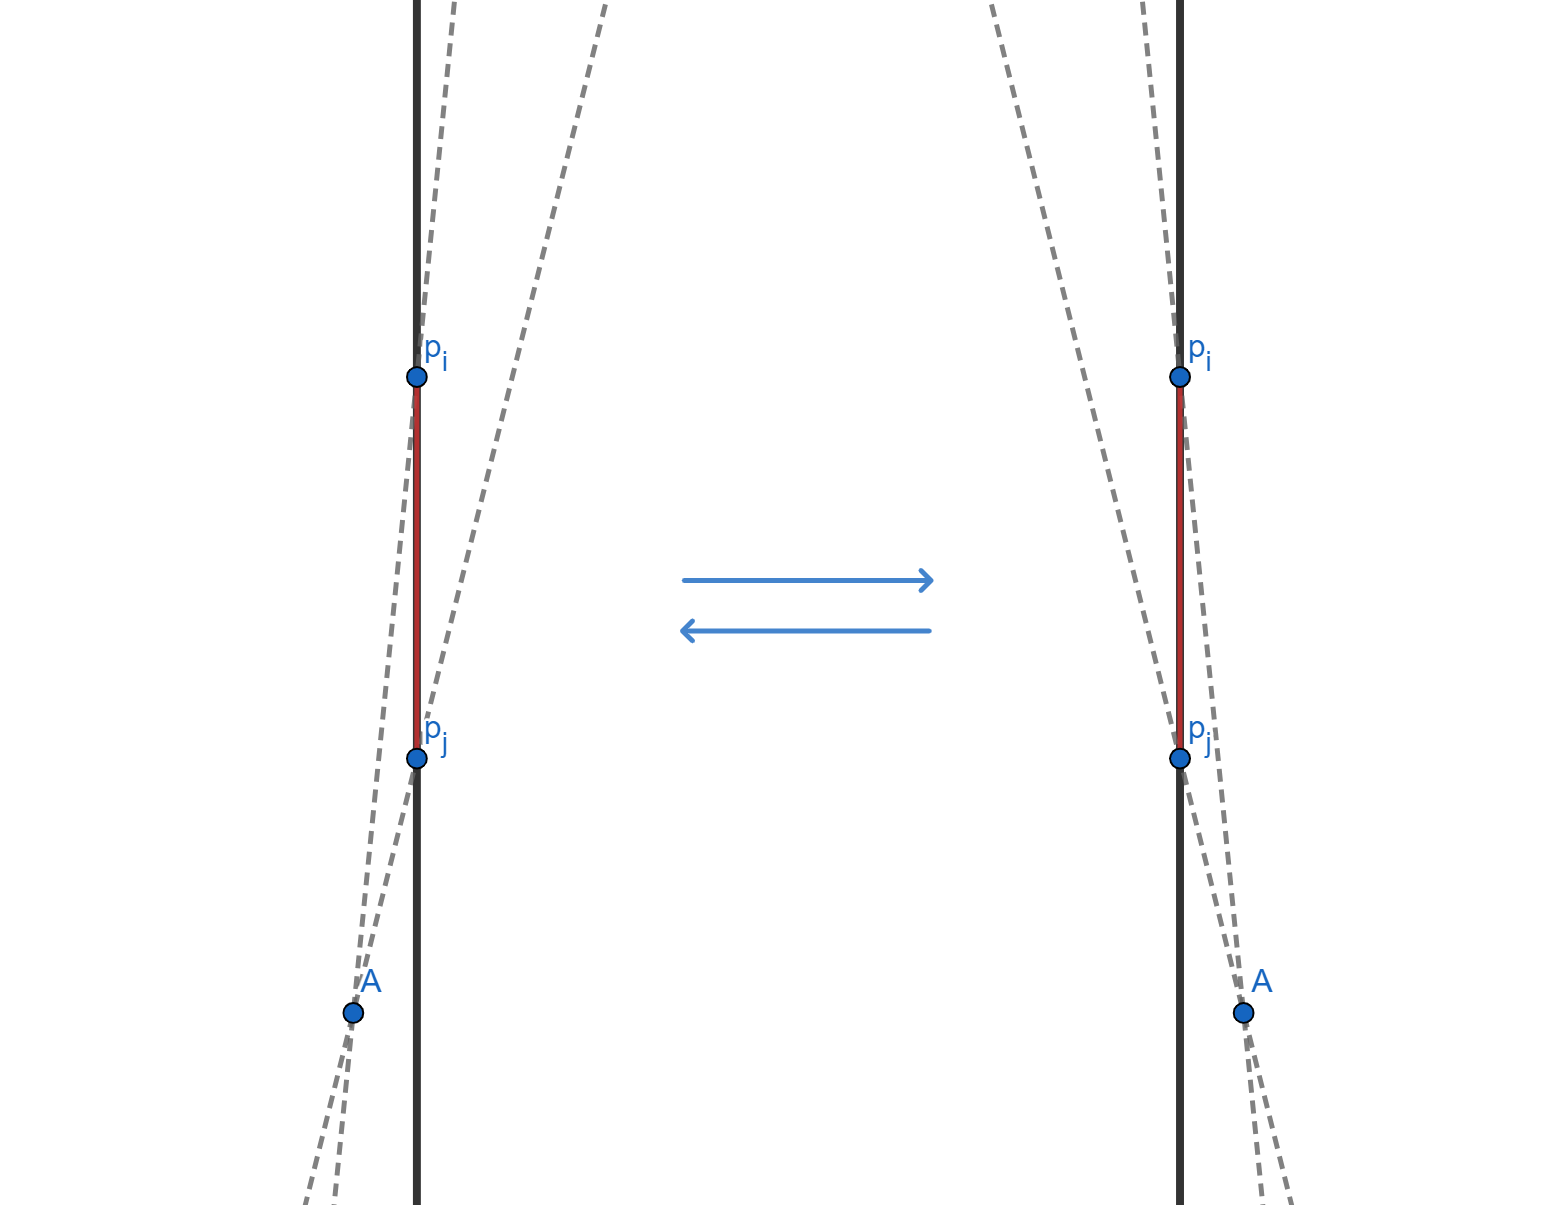
\includegraphics[width=.5\linewidth]{one_segment.png}
            \end{figure}
      \item Точки $p_i, p_j$ лежат на прямой с одной стороны относительно
            <<перешагиваемого>> ребра. Возможны варианты, изображенные ниже,
            а также зеркальные к ним.
            
            Всего 6 случаев достойных рассмотрения (3 пары до-после).
            Точки $p_i, p_j$ в любом случае меняются местами в массиве,
            приведем таблицу изменения правильности 
            ($+$ -- правильный, $-$ -- неправильный):
            
            \begin{center}
                  \begin{tabular}{| c | c | c | c | c |}
                        \hline
                        & верхний-справа & нижний-справа & 
                        верхний-слева & нижний-слева \\
                        \hline
                        Рис. 1 & $+$ & $-$ & $-$ & $-$ \\
                        \hline
                        Рис. 2 & $-$ & $-$ & $-$ & $+$ \\
                        \hline
                        Рис. 3 & $-$ & $-$ & $+$ & $+$ \\
                        \hline
                  \end{tabular}
            \end{center}
            
            По таблице видно, что, если среди рассматриваемых отрезков есть
            хоть один правильный, то оба становятся неправильными после 
            перехода. 
            
            Оставшиеся 3 перехода с двух неправильных отрезков
            можно различить положением отрезков относительно исходной грани:
            \begin{enumerate}
                  \item Отрезки и грань находятся в разных полуплоскостях,
                        относительно ребра.
                  \item Отрезки и грань находятся в одной полуплоскости,
                        относительно ребра.
                  \item Отрезки находятся в разных полуплоскостях,
                        относительно ребра.
            \end{enumerate}
            
            \begin{figure}[H]
                  \centering
                  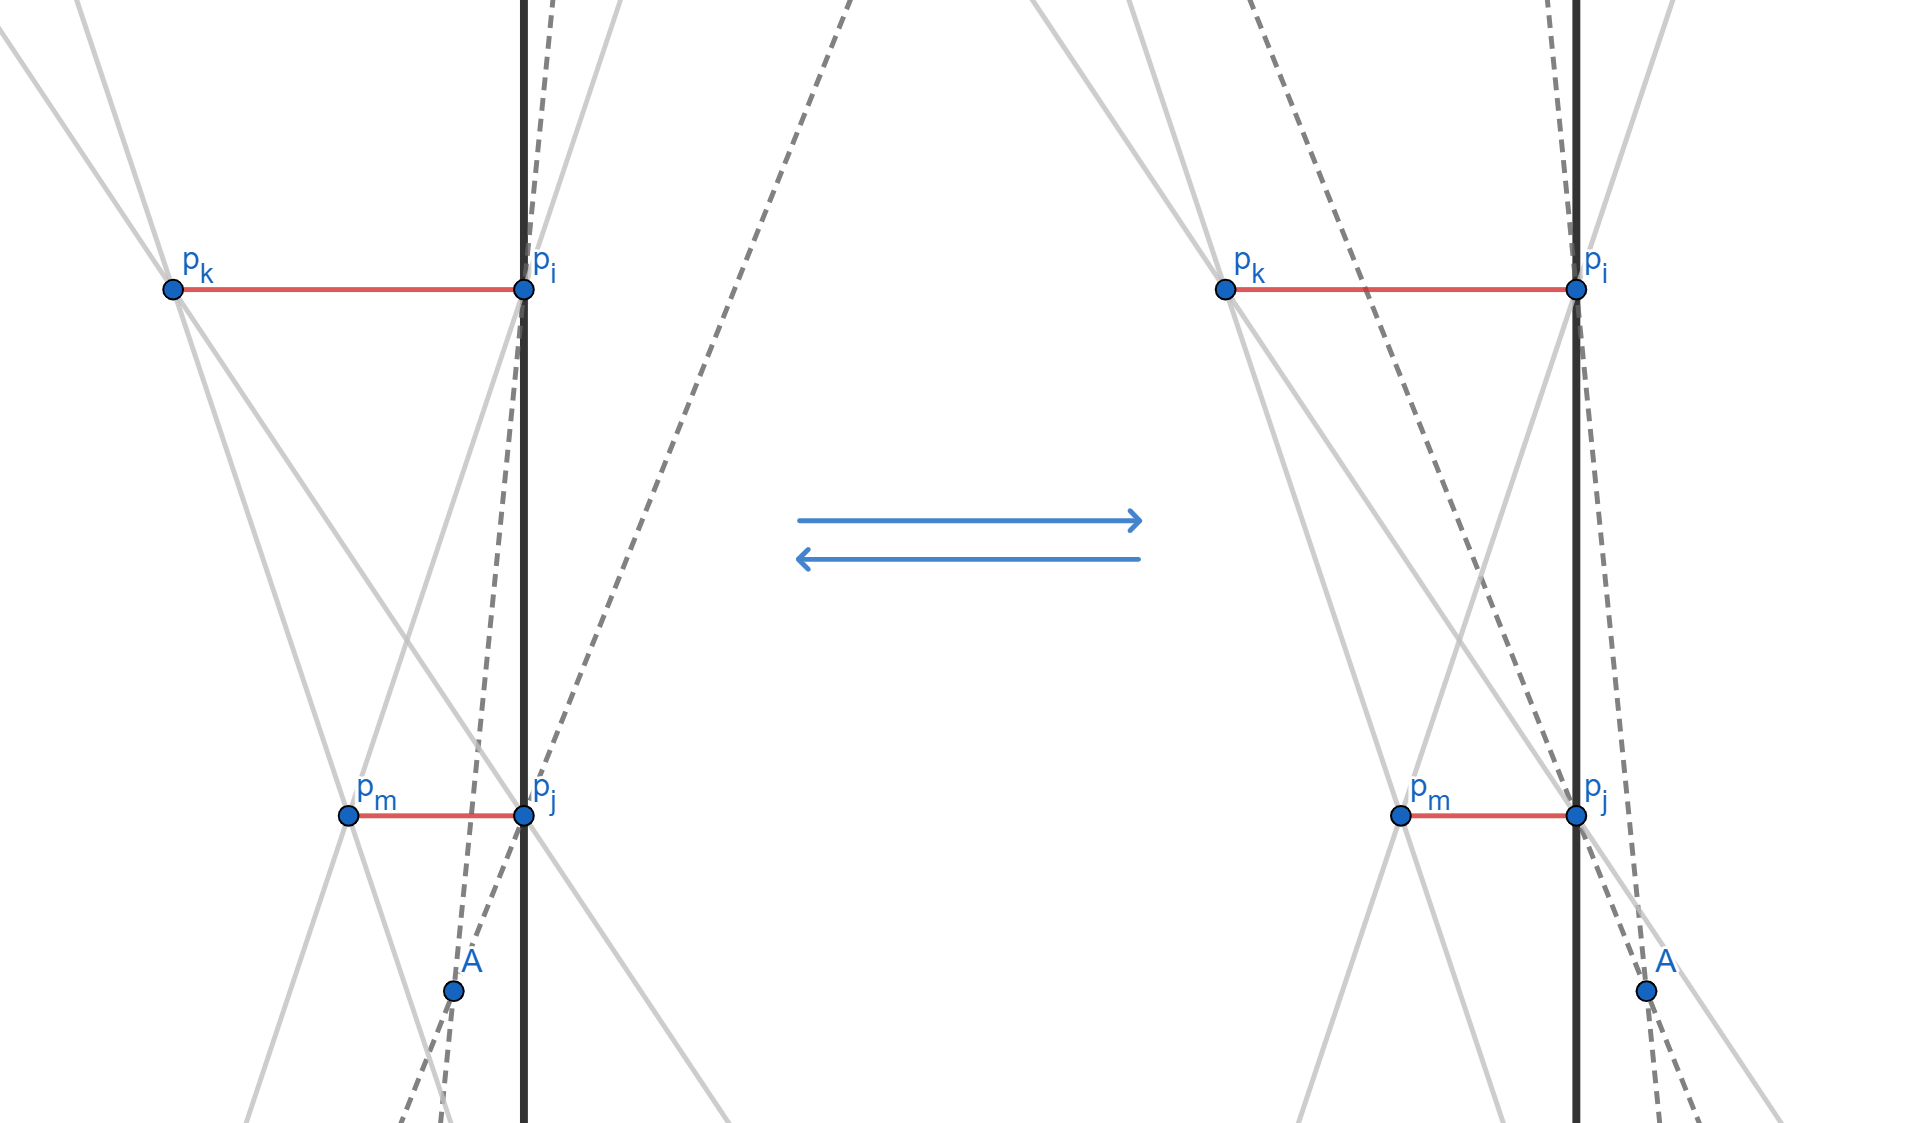
\includegraphics[width=.6\linewidth]{one_side_1.png}
            \end{figure}

            \begin{figure}[H]
                  \centering
                  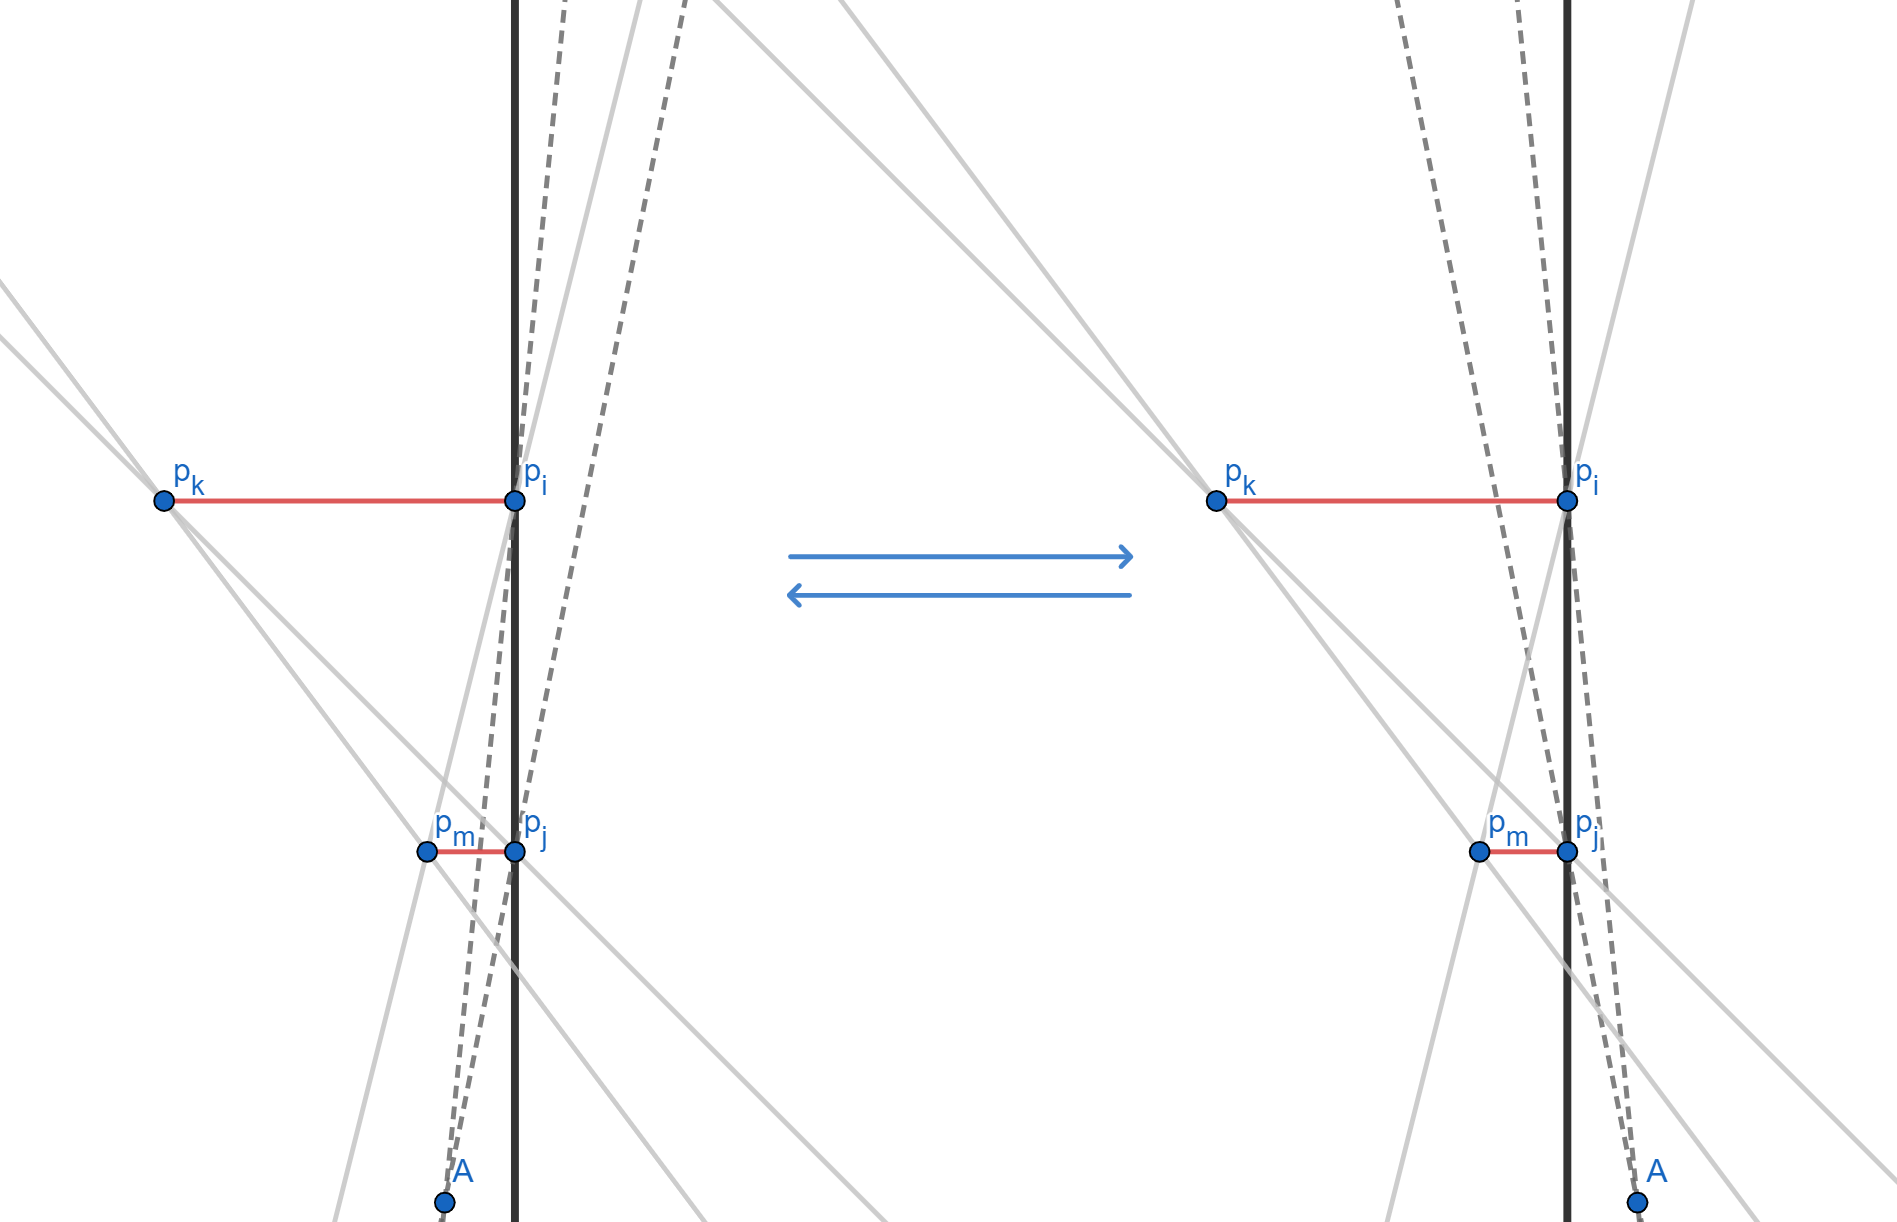
\includegraphics[width=.6\linewidth]{one_side_3.png}
            \end{figure}

            \begin{figure}[H]
                  \centering
                  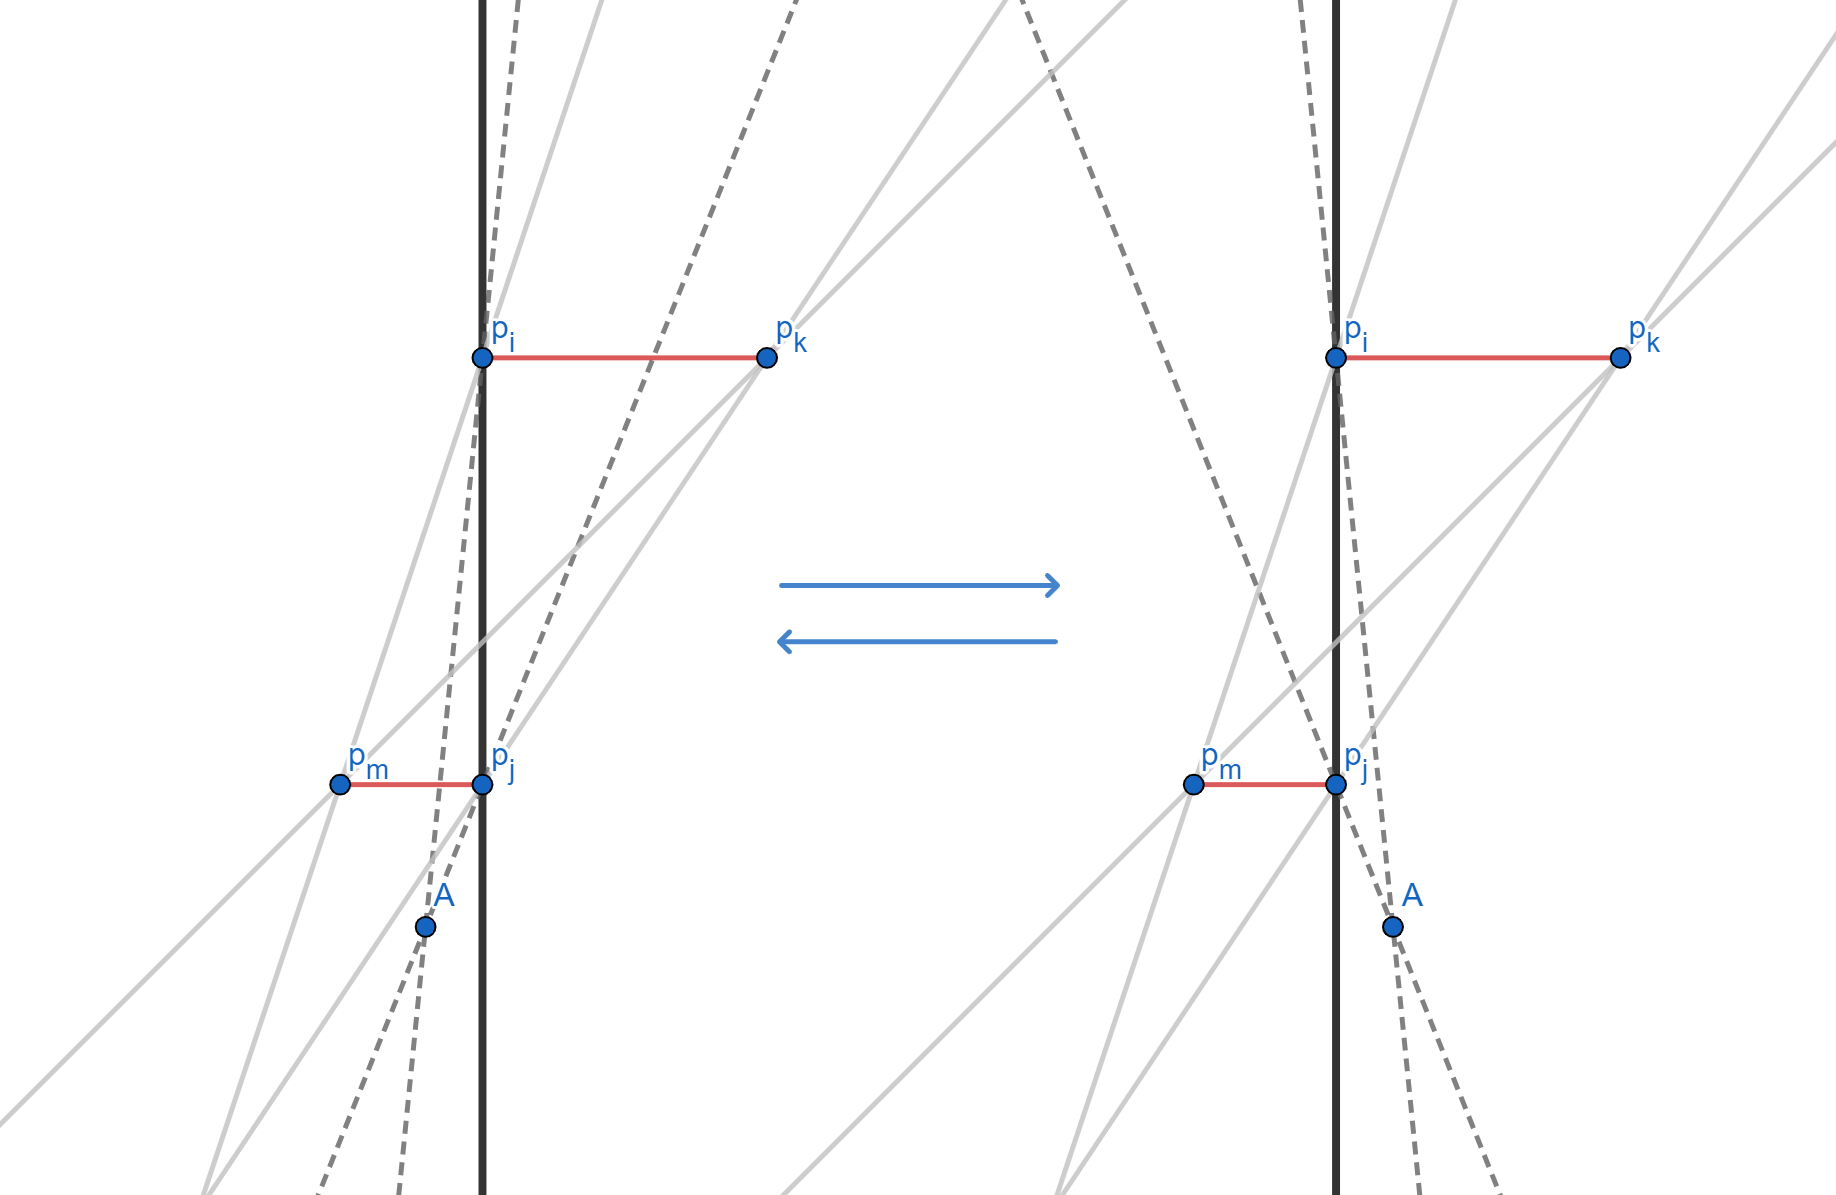
\includegraphics[width=.6\linewidth]{one_side_2.png}
            \end{figure}

      \item Точки $p_i, p_j$ лежат на прямой по разные стороны 
            относительно <<Перешагиваемого>> ребра. Возможны варианты, 
            изображенные ниже, а также зеркальные к ним.
            
            Действие -- без изменений.
            \begin{figure}[H]
                  \centering
                  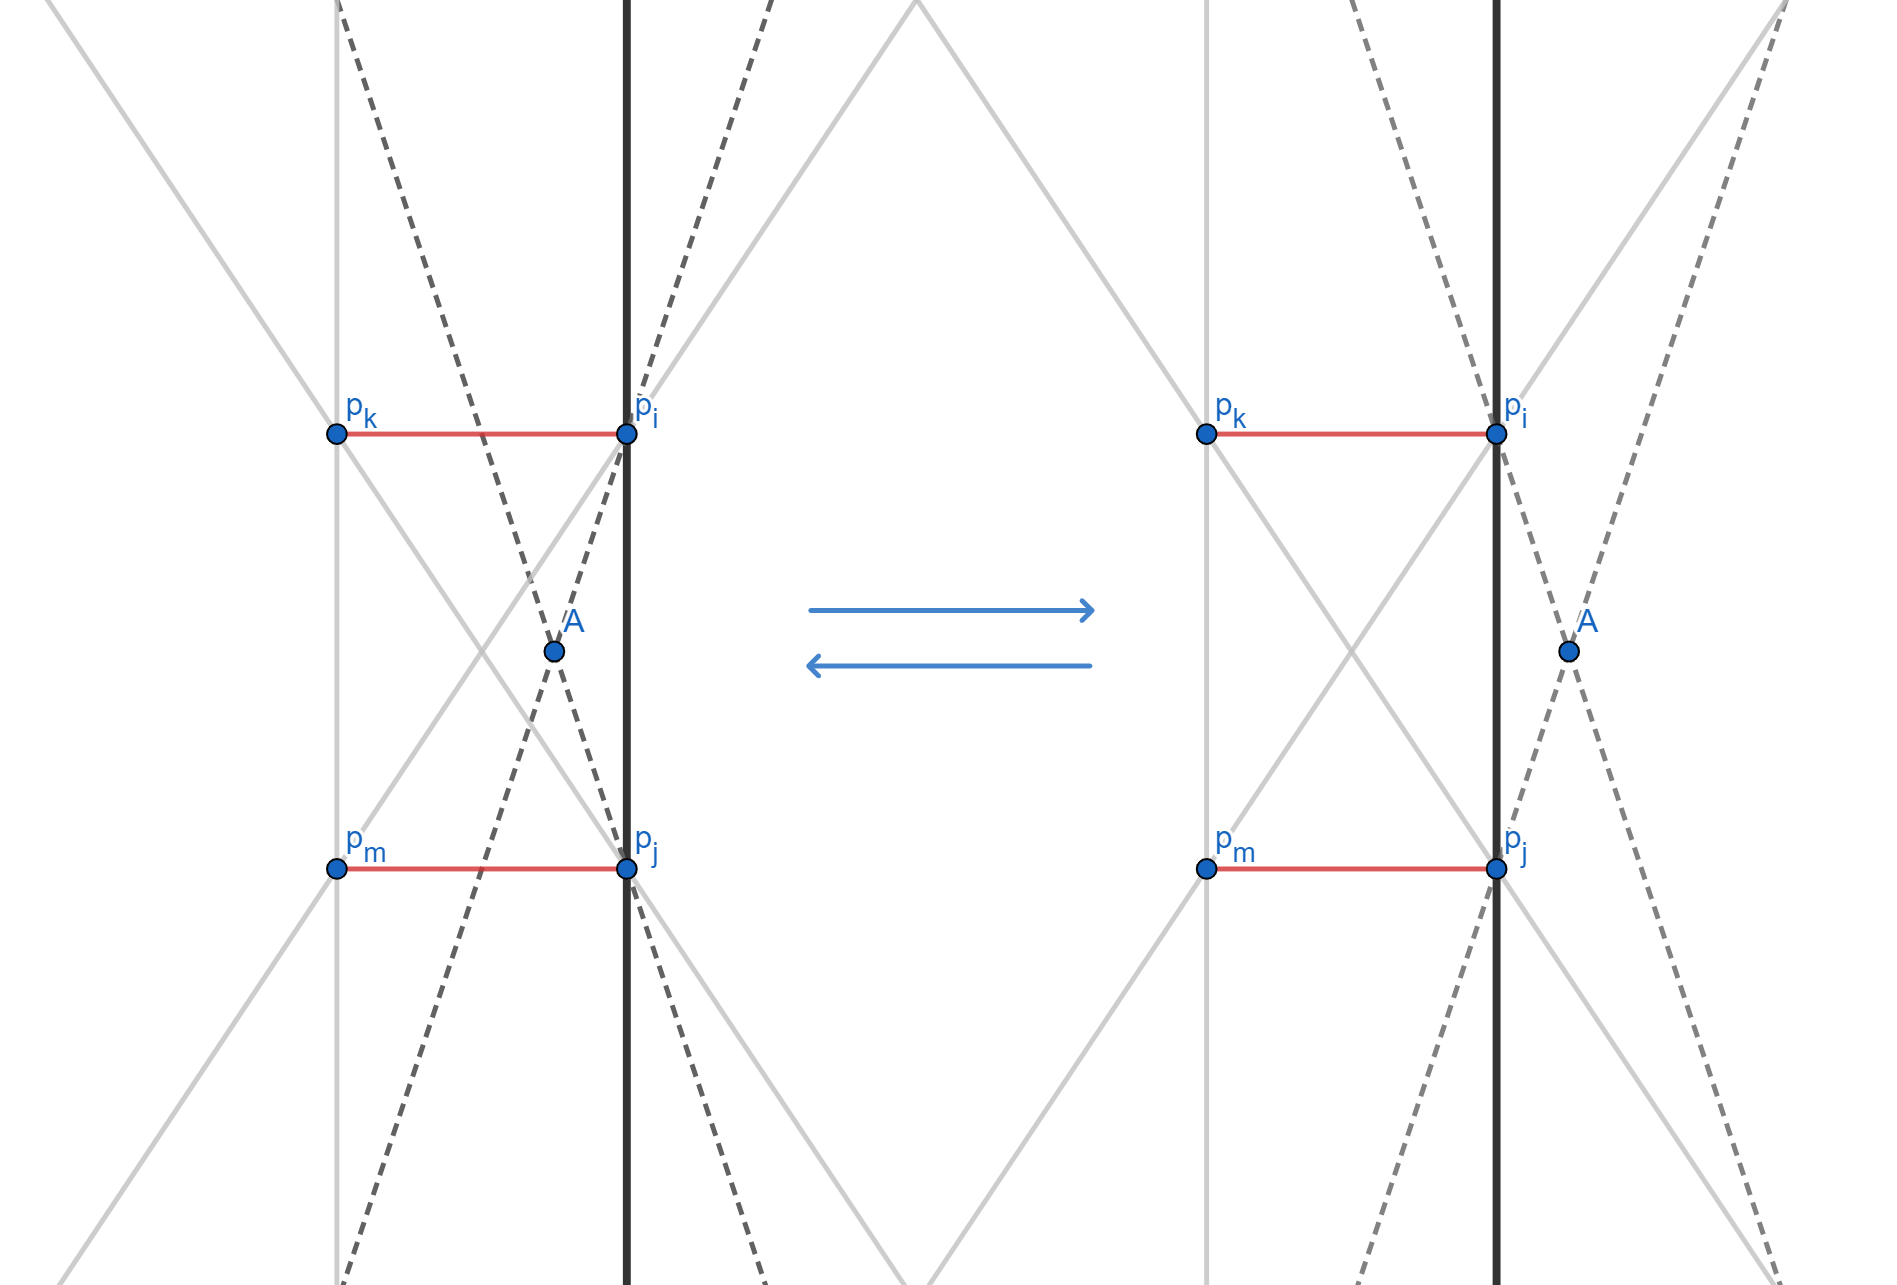
\includegraphics[width=.6\linewidth]{between_1.png}
            \end{figure}
            \begin{figure}[H]
                  \centering
                  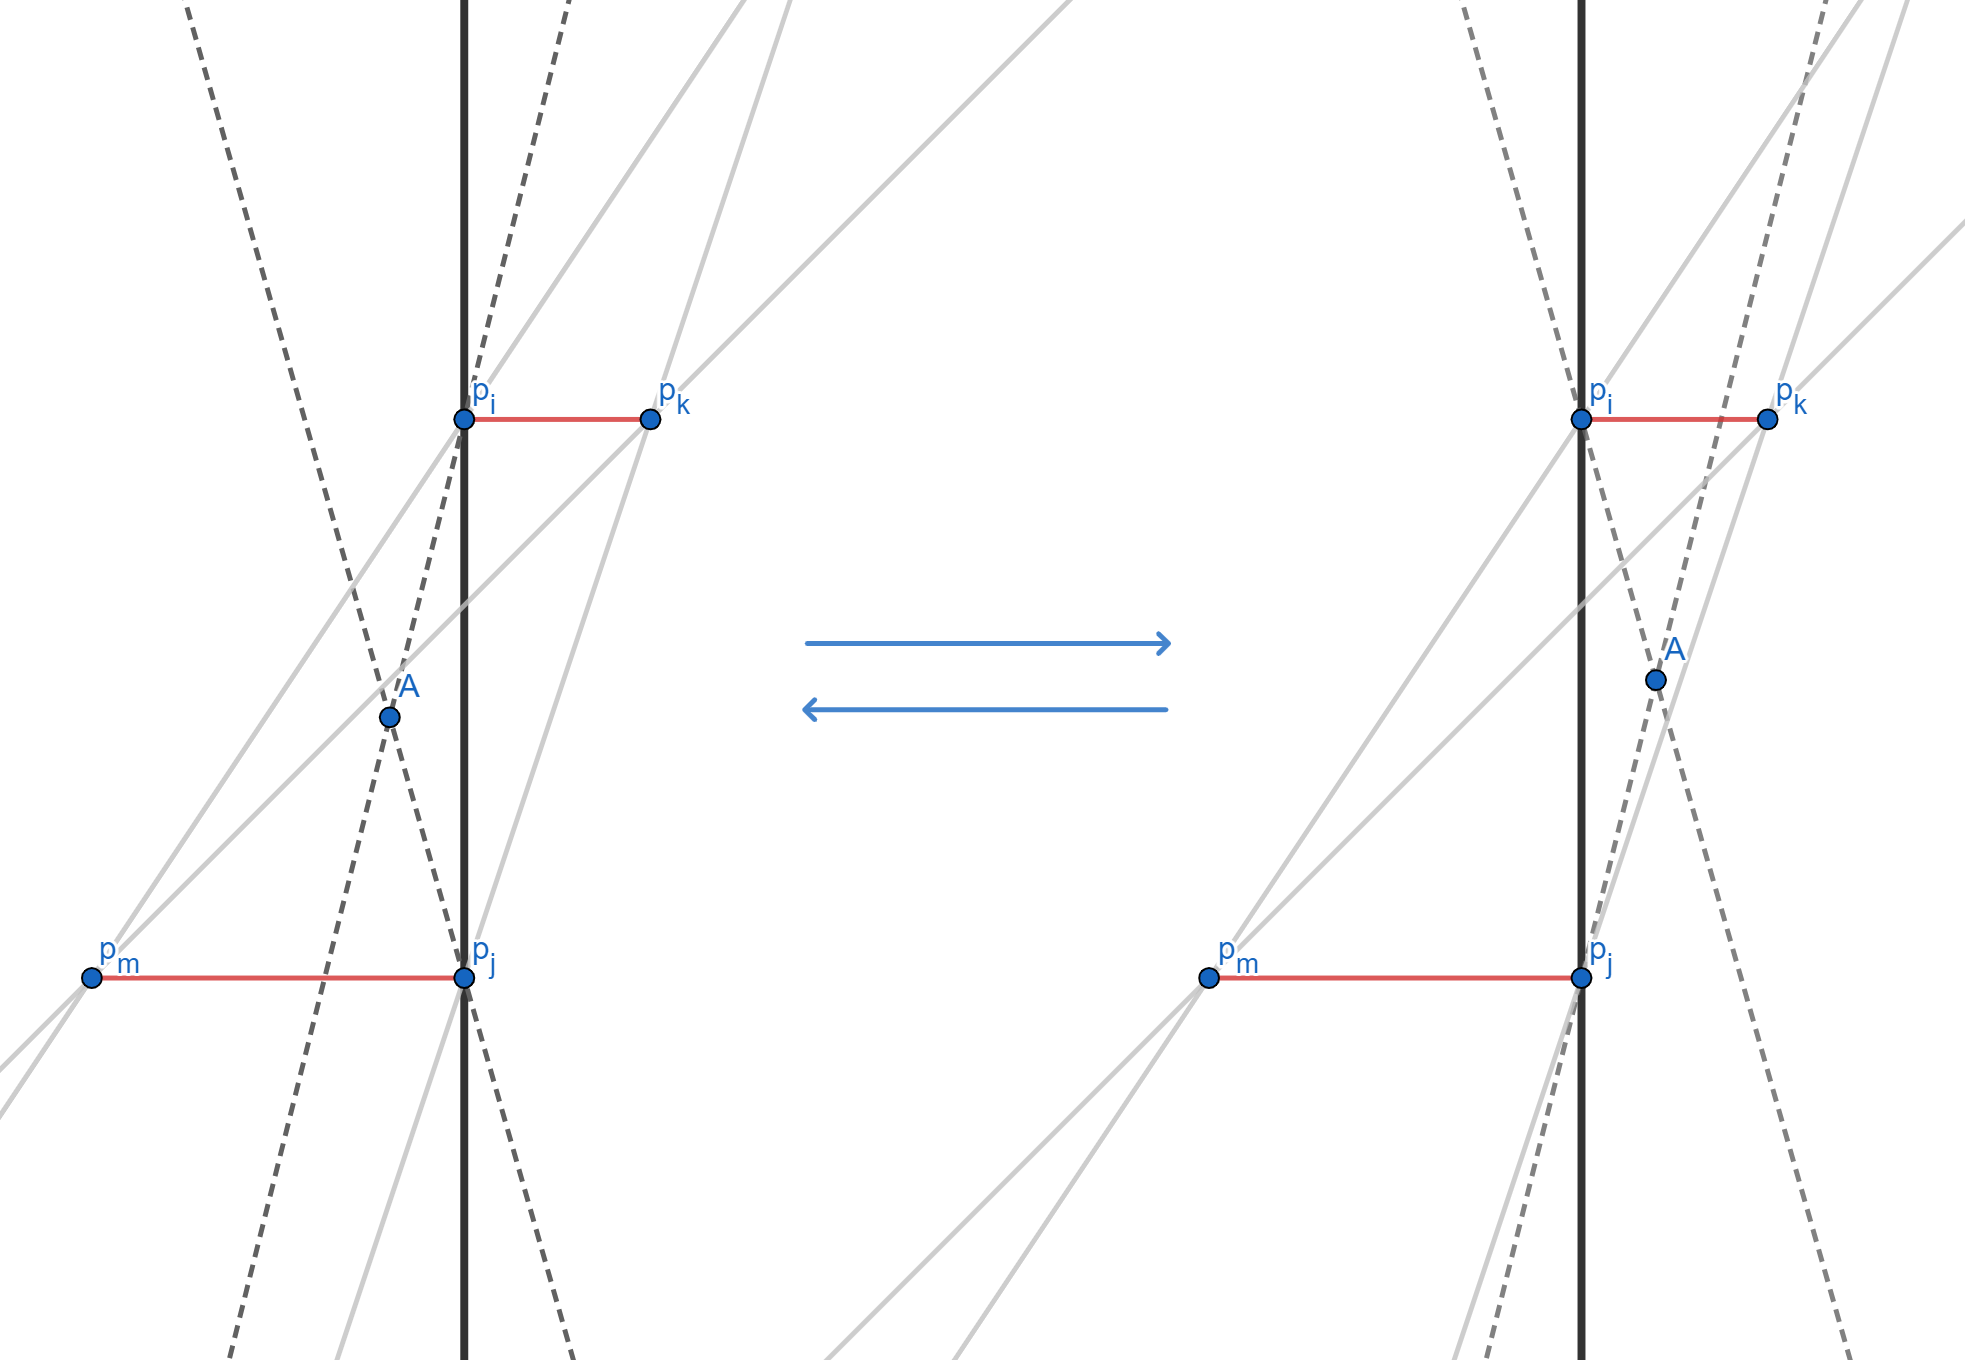
\includegraphics[width=.6\linewidth]{between_2.png}
            \end{figure}
\end{enumerate}
\end{document}